

%%%%%
%%%%% before you you do anything else ...
%%%%%

%%%%% put your last name inside the curly brackets
\def\StudLastName{Bauckhage}

%%%%% put your first name inside the curly brackets
\def\StudFirstName{Christian}

%%%%% put your Matr.-Nbr. inside the curly brackets
\def\StudID{123456789}


%%%%%
%%%%% super important for B-IT students
%%%%%

%%%%% if you are enrolled with B-IT,
%%%%% switch this flag from 0 to 1
\def\BITstudent{0}

%%%%%
%%%%%
%%%%%










\documentclass[12pt,a4paper,fleqn]{report}

%%% packages for mathematical typesetting
\usepackage{amsmath}
\usepackage{amssymb}
\usepackage{times}
\usepackage{bm}
%%% package for inclusing figures
\usepackage{graphicx}
%%% package for nicer table layout
\usepackage{booktabs}
%%% package for color mangement
\usepackage[svgnames]{xcolor}
%%% package for page headings and footers
\usepackage{fancyhdr}

%
% if you include graphics files, LaTeX will search
% for them in the directories specified here 
%
\graphicspath{{./}, {./Figures/}}
%



%
% specifications for page / text layout
% DO NOT EDIT THE FOLLOWING
%
\renewcommand{\familydefault}{\sfdefault}
\pagestyle{fancy}
\cfoot{}
\frenchspacing
\setlength{\headheight}{15pt}
\def\thesection{\arabic{section}.}
\setlength{\parindent}{0pt}
%



%%% vectors, matrices, and tensors
\renewcommand{\vec}[1]{\bm{#1}}
\newcommand{\mat}[1]{\bm{#1}}

%%% sets
\newcommand{\set}[1]{\mathcal{#1}}

%%% probability and conditional probability
\newcommand{\prob}[1]{p\bigl( #1 \bigr)}
\newcommand{\cprob}[2]{p\bigl( #1 \bigm| #2 \bigr)}

%%% typesetting python code
\usepackage{fancyvrb} 
\usepackage{listings}
\lstdefinestyle{Python}{%
	language=Python,
	tabsize=4,
	basicstyle=\ttfamily,
	stringstyle=\color{ForestGreen},
	keywordstyle=\color{BlueViolet},
	commentstyle=\itshape\color{DarkRed!90},
	identifierstyle=,
	emphstyle=\color{Blue},
	frame=none,	
	showstringspaces=false,
	morekeywords={range, len, self, lambda, from, import, as, False, True, enumerate, xrange, 
	              map, list, set, float, int, min, max, sorted, None},
	fancyvrb=true,
}
\lstnewenvironment{PythonCode}[1][]{\lstset{style=Python,#1}}{}





\begin{document}


%%%%%
%%%%% DO NOT EDIT THIS FILE
%%%%%



\lhead{\small \emph{Game AI, ``test'' exam, 2020}}
\rhead{\small \emph{page } \thepage}



Name: \textcolor{blue}{\StudLastName, \StudFirstName}
\hfill
Signature: \underline{\hspace{4cm}}

\vspace{1cm}
MatNr: \textcolor{blue}{\StudID}
\hfill
\begin{minipage}{5.9cm}
  \small
  \if\BITstudent1
  (\textcolor{blue}{X}) student at B-IT / RWTH Aachen \\
  (\textcolor{white}{X}) student at University of Bonn
  \else
  (\textcolor{white}{X}) student at B-IT / RWTH Aachen \\
  (\textcolor{blue}{X}) student at University of Bonn
  \fi
\end{minipage}
\vspace{2cm}



\begin{center}
  
  {\large University of Bonn, B-IT}\\[2ex]
  
  {\large Game AI}
  
  Instructor: Prof. Dr.-Ing. Christian Bauckhage\\[1ex]
  
  ``test'' exam
\end{center}



\textbf{Note:} This is just a text exam \ldots in the real exam on Jul 16th, you will find administrative guidelines at this point. The following table is just a place holder.



\vfill
\begin{center}
  for instructor's use\\[1ex]
  
  \begin{tabular}{ccc}
    \toprule
    problem & points &  score \\
    \midrule
    1 & 10  & \\
    \midrule
    2 & 12 & \\
    \midrule
    3 & 8 & \\
    \midrule
    4 & 10 & \\
    \bottomrule
  \end{tabular}
  \hspace{1cm}
  \begin{tabular}{ccc}
    \toprule
    problem & points & score \\
    \midrule
    5 & 10 & \\
    \midrule
    6 &  8 & \\
    \midrule
    7 & 10 & \\
    \midrule
    8 & 12 & \\
    \bottomrule
  \end{tabular}
  
  \vspace{1cm}
  
  \begin{tabular}{cc}
    \toprule
    total score & $\qquad$ \\
    \bottomrule
  \end{tabular}
\end{center}
\newpage

\textbf{Problem 1:} stochastic processes
\begin{itemize}
\item[a)] [\textbf{2 points}] What is a stochastic process over a discrete, finite state space $\set{S} = \{ s_1, s_2, \ldots, s_m \}$ ? \\[4ex]
%%%%%
%%%%% enter your answer here
%%%%%
A set of random variables $\bigl\{ X_t \bigm| t \in \mathbb{N} \bigr\}$ where $X_t \in \set{S}$.





\vspace{8ex}
\item[b)] [\textbf{2 points}] What is a discrete time Markov chain (DTMC) ? \\[4ex]
%%%%%
%%%%% enter your answer here
%%%%%
A stochastic process such that for all $t \in \mathbb{N}$
\begin{equation*}
\cprob{X_t}{X_{t-1}, \ldots, X_0} = \cprob{X_t}{X_{t-1}} 
\end{equation*}
\end{itemize}
\newpage










\textbf{Problem 2:} Monte Carlo integration
\begin{itemize}
\item[a)] [\textbf{4 points}] Plot the gamma function
\begin{equation*}
\Gamma(z) = \int_0^\infty x^{z-1} \, e^{-x} \, dx
\end{equation*}
for $z \in \{ 1, 2, 3, 4, 5 \}$. \\[2ex]
%%%%%
%%%%% enter your answer here
%%%%%

\begin{center}
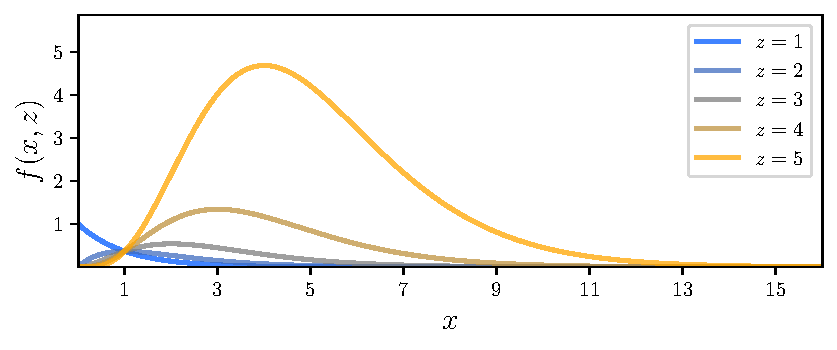
\includegraphics[width=0.9\textwidth]{gamma-integrant.pdf}
\end{center}





\vspace{8ex}
\item[b)] [\textbf{4 points}] Fill in the following table. \\[4ex]
%%%%%
%%%%% enter your answer here
%%%%%

\begin{center}
\begin{tabular}{c@{\hspace{3ex}}c@{\hspace{3ex}}c}
\toprule
$z$ & $(z-1)!$ & $\Gamma(z)$ \\
\midrule
$2$ & 1   & 1 \\
$3$ & 2   & 2 \\
$4$ & 6   & 6\\
$5$ & 24  & 24\\
$6$ & 120 & 120\\
\bottomrule
\end{tabular}
\end{center}





\newpage
\item[b)] [\textbf{4 points}] Show your python code for computing the entries of the above table. \\[4ex]
%%%%%
%%%%% enter your answer here
%%%%%
\begin{PythonCode}
import scipy as sp

for z in [2,3,4,5,6]:
	fact = sp.special.factorial(z-1)
	gamm = sp.special.gamma(z)
	print (fact, gamm)
\end{PythonCode}
\end{itemize}

\end{document}
